\documentclass[10pt,letter]{article}
\usepackage[utf8]{inputenc}
\usepackage[spanish,es-noshorthands]{babel}
\usepackage{amsmath}
\usepackage{amsfonts}
\usepackage{amssymb}
\usepackage{anysize}
\usepackage{soul}
\usepackage{dsfont}
\usepackage{color}
\usepackage{pgfplots}
\usepackage{multicol}
\usepackage{cancel}
\usepackage{titlesec}
\usepackage{float}
\usepackage[tablename=Tabla]{caption}

%Margenes modificables   \begin{changemargin}{-1cm}{-1cm}   ---     \end{changemargin}

\newenvironment{changemargin}[2]{%
\begin{list}{}{%
\setlength{\topsep}{0pt}%
\setlength{\leftmargin}{#1}%
\setlength{\rightmargin}{#2}%
\setlength{\listparindent}{\parindent}%
\setlength{\itemindent}{\parindent}%
\setlength{\parsep}{\parskip}%
}%
\item[]}{\end{list}}

%Titulo y Autores
\title{Caracterización de circuitos RC}
\date{\small{28 de mayo de 2019}}
\author{A. P. Vargas López, D. F. Ortiz Gutierrez, J. C. Prada Sierra \\ \\
\small {Dpto. de Física}\\
\small {Universidad Nacional de Colombia}\\}
\marginsize{2.5cm}{2.5cm}{1cm}{1cm} 


%Formatos de titulo de secciones
\titleformat{\section}[hang]
{\normalfont\bfseries}
{\thesection.}{0.5em}{}

\titleformat{\subsection}[hang]
{\normalfont\bfseries}
{\thesubsection.}{0.5em}{}

\titleformat{\subsubsection}[hang]
{\normalfont\bfseries}
{\thesubsubsection.}{0.5em}{}


%Separacion de Columnas

\setlength{\columnsep}{0.7cm}

\parindent=0.5cm

\begin{document}
\maketitle 

\parindent=0cm
\hrulefill
\parindent=0.5cm

\begin{changemargin}{0.5cm}{0.5cm}

\titleformat{\section}[display]
{\filcenter\normalfont\bfseries}
{\thesection.}{0.5em}{}




\section*{Resumen}
%-----------------------------------------------------------------------------------------------------
%-----------------------------------------------------------------------------------------------------
Los capacitores son componentes eléctricos con diversas y variadas aplicaciones en distintos campos de las ciencias e ingenierías [Aqui deberiamos colocar alguna referencia que hable sobre aplicaciones de capacitores], son bases de la electrónica moderna y su estudio es fundamental para mostrar sus características más destacables. En este trabajo se explorarán los conceptos básicos referentes a capacitores como lo son: su disposición en serie y en paralelo a través de las reglas para obtener capacitancias equivalentes y su comportamientos al combinarse en un mismo circuito con resistencias. Durante el proceso se logró respaldar la formulación teórica de los objetos estudiados de forma experimental, mediante el uso de herramientas sencillas como voltimetros y amperimetros así como con instrumentos más precisos como el osciloscopio digital. El resultado más destacable obtenido con el osciloscopio muestra el comportamiento de carga y descarga de los circuitos RC.

\vspace{0.5cm}

\parindent=0cm
\hrulefill
\parindent=0.5cm


\end{changemargin}
%-----------------------------------------------------------------------------------------------------
%-----------------------------------------------------------------------------------------------------


\vspace{1cm}


\titleformat{\section}[hang]
{\normalfont\bfseries}
{\thesection.}{0.5em}{}

\begin{multicols}{2}
\section{Introducción}

\subsection{¿Qué es un capacitor?}

Un capacitor o condensador es un dispositivo que permite almacenar energía debido a que puede generar una diferencia de potencial entre dos placas conductoras paralelas que posee en su interior. Al cargarlas en igual magnitud, pero cada una con signo opuesto, se genera un campo eléctrico y por ende una diferencia de potencial entre ellas. Dichas placas vienen separadas por un aislante o simplemente el vacío para evitar la transferencia de carga entre ellas.

\vspace{0.2cm}

A partir de esto se puede definir la Capacitancia ($C$) como la capacidad de un componente o circuito para recoger y almacenar energía en forma de carga eléctrica ($Q$). Su unidad de medida es el Faradio ($F$). La diferencia de potencial de un capacitor viene dada por:
\begin{equation}
V=\dfrac{Q}{C}
\end{equation}
\subsection{Capacitores en serie y en paralelo}

Al conectar un capacitor a una fuente o batería, este se cargará hasta que sus placas adquieran la misma diferencia de potencial entre ellas que el que genera la fuente. En el caso de un circuito sencillo con $n$ capacitores en serie, la suma de sus respectivas diferencias de potencial será igual a la diferencia de potencial de la fuente. De esto se deduce que la capacitancia equivalente del circuito es:
\begin{equation}
C_{eq}=\left(\dfrac{1}{C_1}+\dfrac{1}{C_2}+\dots+\dfrac{1}{C_n}\right)^{-1}
\end{equation}
Esto porque la carga en cada uno de los $n$ capacitores en serie sera la misma, al igual que la carga considerada para el capacitor equivalente, es decir:
\begin{equation}
Q_{total}=Q_1=Q_2=\dots=Q_n
\end{equation}
Sin embargo, si los $n$ capacitores están en paralelo, el voltaje será el mismo para la fuente y para cada capacitor; pero la carga total en el circuito será igual a la suma de las cargas almacenadas por cada capacitor. De esto se obtiene que para este caso la capacitancia equivalente del circuito es:
\begin{equation}
C_{eq}=C_1+C_2+\dots+C_n
\end{equation}
Para descargar el capacitor basta con apagar la fuente del circuito. En seguida, las cargas se empezarán a redistribuir buscando el equilibrio electrostático.

\subsection{Carga y descarga del circuito RC}

\begin{figure}[H]
\centering
\resizebox{6cm}{3cm}{	
	\begin{tikzpicture}
		\draw [scale=1] (0,-0.05)--(0,-1)--(3,-1)--(3,-0.5)--(3.1,-0.4)--(2.9,-0.3)--(3.1,-0.2)--(2.9,-0.1)--(3.1,0)--(2.9,0.1)--(3.1,0.2)--(2.9,0.3)--(3.1,0.4)--(3,0.5)--(3,1)--(1.55,1);
		\draw [scale=1] (0,0.05)--(0,1)--(1.45,1);
		%Bateria
		\draw [thick, scale=1] (-0.25,-0.05)--(0.25,-0.05);
		\draw [thick, scale=1](-0.2,0.05)--(0.2,0.05);
		%Capacitor
		\draw [thick, scale=1](1.55,1.2)--(1.55,0.8);
		\draw [thick, scale=1](1.45,1.2)--(1.45,0.8);
		
		\draw [scale=1](-0.3,0) node[left]{$V_0$};
		\draw [scale=1](1.5,1.3) node[above]{$C$};
		\draw [scale=1](3.3,0) node[right]{$R$};
		\draw [scale=1](0.4,-0.08)node[right]{$+$};
		\draw [scale=1](0.4,0.08)node[right]{$-$};
	\end{tikzpicture}
}
\caption{Circuito RC básico en proceso de carga}
\label{RCcarga}
\end{figure}

Ahora consideremos el proceso de carga de un circuito RC como el de la figura 1, por suma de diferencias de potencial en un camino cerrado sabemos que, para una fuente de voltaje $V_0$, resistencia $R$ y capacitancia $C$ se tiene: 

$$IR+\dfrac{q}{C}-V_0=0$$
$$\text{Puesto que } I=\dfrac{dq}{dt} \text{, entonces}$$
$$RC\dfrac{dq}{dt}=CV_0-q$$
$$\int_0^{q(t)}\dfrac{dq}{q-CV_0}=\int_0^t\dfrac{-dt}{RC}$$
$$ln(q-CV_0)|_0^{q(t)}=-\dfrac{t}{RC}$$
$$ln\left(\dfrac{q(t)-CV_0}{-CV_0}\right)=-\dfrac{t}{RC}$$
$$\dfrac{q(t)-CV_0}{-CV_0}=e^{-\frac{t}{RC}}$$
$$q(t)=CV_0\left(-e^{-\frac{t}{RC}}\right)$$
$$\text{Puesto que } V=\dfrac{q}{C} \text{ en el capacitor, se tiene que:}$$ 
\begin{equation}
V(t)=V_0\left(1-e^{-\frac{t}{RC}}\right)
\end{equation}

Lo cual es el voltaje en el capacitor en funcion del tiempo

\vspace{0.3cm}

Una vez ha pasado un tiempo lo suficientemente largo, lo suficiente para considerar que el capacitor tiene una diferencia de potencial $V_0$ y quitamos la fuente del circuito en la figura 1 tendremos un circuito formado exclusivamente por resistencia y capacitor, lo cual generará la descarga del capacitor dada por:

$$\dfrac{dq}{dt}R+\dfrac{q}{c}=0$$
$$\dfrac{dq}{dt}=-\dfrac{q}{RC}$$
$$\int_{CV_0}^{q(t)}\dfrac{dq}{q}=\int_0^t\dfrac{dt}{RC}$$
$$ln\left(\dfrac{q(t)}{CV_0}\right)=-\dfrac{t}{RC}$$ 
$$\dfrac{q(t)}{C}=V_0e^{-\frac{t}{RC}}$$
\begin{equation}
V(t)=V_0e^{-\frac{t}{RC}}
\end{equation}

\subsection{El tiempo característico $\tau$ }

El denominado Tiempo Característico del Circuito $\tau$ es importante para determinar que tan rápido se carga y descarga un capacitor en un circuito RC en comparación a otros con determinada resistencia R. Este se define como:
\begin{equation}
\tau=RC
\end{equation}
Es decir que cuando ha pasado el tiempo $\tau$ en el circuito RC en descarga, el voltaje en el capacitor será:
\begin{equation}
V(\tau)=\dfrac{V_0}{e}
\end{equation}

\subsection{•}

%-----------------------------------------------------------------------------------------------------
%-----------------------------------------------------------------------------------------------------

\section{Dispositivo experimental y procedimiento}
La práctica de laboratorio se encuentra separada en dos procedimientos cuya principal diferencia es el equipo utilizado y la precisión que este permite. 

El primer procedimiento se busca medir el tiempo característico $\tau$ de un circuito RC en descarga mediante un multímetro y cronómetro, esto para calcular el valor de la resistencia utilizada en el circuito ya que se conocía el valor de la capacitancia. Así mismo se comprobó la capacitancia equivalente de un montaje en serie de capacitores. 

El segundo procedimiento consistió en utilizar un osciloscopio para medir el tiempo $\tau$ de un circuito RC con tiempos de carga y descarga del orden de los microsegundos. Esto fue utilizado para calcular el valor de los capacitores utilizados a partir de distintas resistencias. Cada uno de los procedimientos es explicado en profundidad a continuación.

\subsection{Procedimiento 1}
\subsubsection{Equipo y materiales}
Equipo utilizado para la medición de $\tau$ en distintos circuitos RC y la capacitancia equivalente  para capacitores en serie:
\begin{enumerate}
\itemsep=0em
\item Capacitores ($C_0,C_1,C_2$).
\item Resistencias cuyo valor se desea encontrar.
\item Multímetro digital Manual YF-3503 AC/DC.
\item Cronómetro con función de vueltas. 
\item Fuente AC/DC PEAK TECH.
\item Caja de capacitores EXTECH de valor modificable ($C_3$).
\item Cables de conexión.
\end{enumerate}

Las capacitancias de los capacitores usados en el procedimiento son especificados en la siguiente tabla.

\begin{table}[H]
\centering
\begin{tabular}{|c|c|}
\hline
\multicolumn{2}{|l|}{Valores de Capacitancias} \\ \hline
Capacitor & $nF$ \\ \hline
$C_0$ & 110.000 \\ \hline
$C_1$ & 544 \\ \hline
$C_2$ & Valor a encontrar \\ \hline
$C_3$ (Caja de Capacitores)& 700 \\ \hline
\end{tabular}
\caption{Valores de capacitancias utilizadas en el procedimiento 1}
\end{table}

\subsubsection{Montaje y procedimiento para encontrar $\tau=RC$}

\begin{figure}[H]
\centering
\resizebox{6cm}{2.2cm}{	
	\begin{tikzpicture}
		\draw [scale=1] (0,-0.05)--(0,-1)--(1.5,-1)--(1.5,-0.5)--(1.6,-0.4)--(1.4,-0.3)--(1.6,-0.2)--(1.4,-0.1)--(1.6,0)--(1.4,0.1)--(1.6,0.2)--(1.4,0.3)--(1.6,0.4)--(1.5,0.5)--(1.5,1)--(1.3,1)--(0.7,1.3);
		\draw [scale=1] (0,0.05)--(0,1)--(0.7,1);
		\draw [scale=1] (1.5,1)--(3,1)--(3,0.05);
		\draw [scale=1] (1.5,-1)--(3,-1)--(3,-0.05);
		\draw [scale=1]	(3,1)--(4.5,1)--(4.5,0.4);
		\draw [scale=1]	(3,-1)--(4.5,-1)--(4.5,-0.4);
		\draw [scale=1]	(4.5,0) circle (0.4);		
		
		%Bateria
		\draw [thick, scale=1] (-0.2,-0.05)--(0.2,-0.05);
		\draw [thick, scale=1](-0.25,0.05)--(0.25,0.05);
		%Capacitor
		\draw [thick, scale=1] (2.8,-0.05)--(3.2,-0.05);
		\draw [thick, scale=1](2.8,0.05)--(3.2,0.05);
		
		\draw [scale=1](4.5,0) node{$V$};		
		\draw [scale=1](-0.3,0) node[left]{$V_0$};
		\draw [scale=1](3.2,0) node[right]{$C$};
		\draw [scale=1](1.6,0) node[right]{$R$};
		\draw [scale=1](0.3,-0.1) node[right]{$-$};
		\draw [scale=1](0.3,0.1) node[right]{$+$};
		\draw [scale=1](2.7,-0.1) node[left]{$-$};
		\draw [scale=1](2.7,0.1) node[left]{$+$};
	\end{tikzpicture}
}
\caption{Circuito RC}
\label{RCcarga}
\end{figure}

El montaje experimental para la medición del tiempo $\tau$ es el mostrado en la figura 2, donde el capacitor utilizado es $C_0$. Al comenzar el experimento se completó el circuito para cargar el capacitor con la diferencia de potencial configurada en la fuente, $V_0=15V$, la cual es mostrada en el multímetro que está dispuesto para medir voltaje, una vez el capacitor está cargado se abre el circuito al mismo tiempo que se comienza a registrar el tiempo con el cronómetro, se observa la medición de voltaje del multímetro  y a intervalos de $0.5V$ de descarga, es decir en $14.5V$,$14V$,$13.5V \dots$ se registra una vuelta en el cronómetro, esto permitió obtener una curva de tiempo vs voltaje. Este procedimiento se llevó a cabo con dos resistencias diferentes $R_1$ y $R_2$, para las cuales se tomaron valores hasta alcanzar voltajes de $1V$ y $4.5V$ respectivamente.

\bigskip

Las incertidumbres en la medición durante este procedimiento fueron:
\begin{enumerate}
\itemsep=0em
\item Multímetro midiendo voltaje: $\pm 0.05V$.
\item Cronómetro: $\pm 0.05s$.
\end{enumerate}

Una vez se tienen las medidas de voltaje en función del tiempo en una gráfica, se encontró el valor $\frac{V_0}{e}$ en el eje de voltaje, se buscó el punto más cercano sobre la curva al cual corresponde dicho valor y dado que la coordenada temporal de dicho punto corresponde al valor de $\tau$ según la ecuación 8, se obtiene $\tau$. Una vez se obtuvo $\tau$ se calculó el valor de cada una de las resistencias por medio de la ecuación 7.


\subsubsection{Montaje de capacitores en serie}

Se realizó el montaje de 3 capacitores en serie conectados a una fuente de $V_0=15V$ tal como se muestra en la figura 3, de estos tres capacitores se conocía el valor de dos de ellos tal como se indica en la tabla 1. Para encontrar la carga en uno de los capacitores con capacitancia conocida se mide la caída de potencial $V_1$ en $C_1$ y se despeja de la ecuación 1 la carga $Q_1$. Se procede ahora a medir la  diferencia de potencial $V_{Total}$ para los tres capacitores con el fin de despejar la capacitancia equivalente $C_{eq}$ del circuito con la ecuación 1; pues la carga total $Q_{total}$ es igual a $Q_1$ por la ecuación 3. A partir de $C_{eq}$, $C_1$ y $C_3$ se reemplaza en la ecuación 2 y se despeja el valor de C2 buscado.


\begin{figure}[H]
\centering
\resizebox{5cm}{4cm}{	
	\begin{tikzpicture}
		\draw [scale=1](-0.1,1)--(-3,1)--(-3,3)--(-2.1,3);
		\draw [scale=1](-1.9,3)--(-0.1,3);
		\draw [scale=1](0.1,3)--(1.9,3);
		\draw [scale=1](2.1,3)--(3,3)--(3,1)--(0.1,1);
		
		\draw [thick,scale=1](-0.1,0.6)--(-0.1,1.4);
		\draw [thick,scale=1](0.1,0.7)--(0.1,1.3);	
		\draw [thick,scale=1](0.1,2.6)--(0.1,3.4);	
		\draw [thick,scale=1](-0.1,2.6)--(-0.1,3.4);
		\draw [thick,scale=1](-1.9,2.6)--(-1.9,3.4);
		\draw [thick,scale=1](-2.1,2.6)--(-2.1,3.4);	
		\draw [thick,scale=1](2.1,2.6)--(2.1,3.4);
		\draw [thick,scale=1](1.9,2.6)--(1.9,3.4);	
		
		\draw [scale=1](-2,2.4) node[below]{$C_1$};				
		\draw [scale=1](0,3.4) node[above]{$C_2$};
		\draw [scale=1](2,2.4) node[below]{$C_3$};
		\draw [scale=1](0,1.45) node[above]{$V_0$};	
		\draw [scale=1](-0.15,0.6)node[below]{$+$};
		\draw [scale=1](0.15,0.6)node[below]{$-$};
		\draw [scale=1](-2,4.5) node{$V_1$};
		\draw [scale=1](0,-0.4) node{\small{$V_{Total}$}};
		
		\draw [scale=1](-2.5,3)--(-2.5,4.5)--(-2.4,4.5);
		\draw [scale=1](-1.5,3)--(-1.5,4.5)--(-1.6,4.5);
		\draw (-2,4.5) circle (0.4);		
		
		\draw [scale=1](-2,1)--(-2,-0.5)--(-0.5,-0.5);
		\draw [scale=1](2,1)--(2,-0.5)--(0.5,-0.5);
		\draw (0,-0.4) circle (0.5);
	
	\end{tikzpicture}
}
\caption{Capacitancias conectadas en serie}
\label{RCcarga}
\end{figure}

La incertidumbre de las medidas de voltaje para este procedimiento es de $\pm0.005V$.


\subsection{Procedimiento 2}
\subsubsection{Equipo y Materiales}
El equipo utilizado para el segundo procedimiento es:

\begin{enumerate}
\itemsep=0em
\item Fuente generadora de corriente OWON A6 1022.
\item Osciloscopio OWON Smart D55032EV.
\item 4 Resistencias (Tabla 2).
\item 2 capacitores de capacitancia desconocida.
\item Cables de conexión.
\item Cables coaxiales.
\end{enumerate}

\begin{table}[H]
\centering
\begin{tabular}{|c|c|}
\hline
\multicolumn{2}{|l|}{Valores de Resistencias} \\ \hline
Resistencia & nF \\ \hline
$R_1$ & 4600 $\pm 5\%$ \\ \hline
$R_2$ & 2200 $\pm 5\%$ \\ \hline
$R_3$ & 1200 $\pm 5\%$ \\ \hline
$R_4$ & 2700 $\pm 5\%$ \\ \hline
\end{tabular}
\caption{Valores de resistencias utilizadas en el procedimiento 2}
\end{table}

\subsubsection{Montaje circuito RC - Fuente - Osciloscopio}

El osciloscopio permite medir oscilaciones de corriente extremadamente cortas en el tiempo con gran precisión, este fue incluido en la medición del circuito RC tal como se muestra en la figura 4 para medir el voltaje en el capacitor pues los tiempos de carga y descarga del circuito son extremadamente cortos para las resistencias y capacitores utilizados, por otro lado la fuente generadora de corriente se utilizó para producir una onda cuadrada con frecuencia 10.000 Hz la cual simula la conexión y desconexión del cirucuito que a su vez genera su carga y descarga en tiempos del orden de microsegundos, esta fuente también se conectó directamente al osciloscopio para observar la relación entre la señal que entraba al circuito y la que se producía en el capacitor.

\begin{figure}[H]
\centering
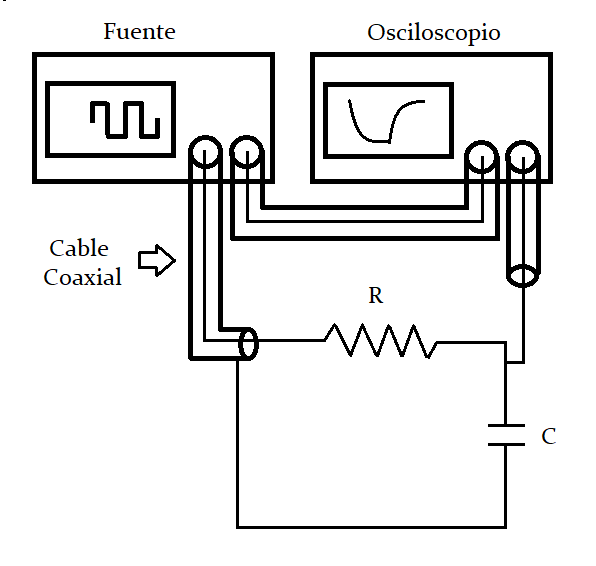
\includegraphics[scale=0.4]{Circuito}
\caption{Circuito RC conectado a fuente generadora y osciloscopio}
\label{RCcarga}
\end{figure}


La fuente se configuró con una diferencia de potencial de pico a pico $V_0=10V$, así, al buscar el valor de $\tau$ en el osciloscopio se buscaba el punto el cual el voltaje en el capacitor tuviera un valor $V(\tau)=\frac{10V}{e}\approx3.67V$ al momento de la descarga.

\vspace{0.2cm}

Este procedimiento de medir $\tau$ es realizado para cada capacitor con cada una de las resistencias, así, para un mismo capacitor se obtuvieron 4 mediciones de $\tau$, uno por cada resistencia, con los cuales calcular su capacitancia por medio de la ecuación 7 y obtener una mejor medida al realizar el promedio. 

\vspace{0.2cm}

Las incertidumbres en las mediciones del osciloscopio son especificadas en la sección de resultados pues para cada resistencia se utilizó una escala diferente y por tanto cada una fue medida con diferente incertidumbre, sin embargo estas se encuentran entre $\pm 10\mu s$ y $\pm 20 \mu s$.






%-----------------------------------------------------------------------------------------------------
%-----------------------------------------------------------------------------------------------------

\section{Resultados y análisis}

%-----------------------------------------------------------------------------------------------------
%-----------------------------------------------------------------------------------------------------

\section{Conclusiones}

%-----------------------------------------------------------------------------------------------------
%-----------------------------------------------------------------------------------------------------

\end{multicols}
\end{document}